\section{Approach}
Plenty of literature exists on modeling both surface rail networks, which typically cover longer distances, and subway or light-rail systems, which typically operate with a higher train frequency. Where simulations of surface rail networks might focus on maintaining arrival and departure schedules, subway and metro systems are more interested in keeping the trains moving and avoiding deadlock.  Deadlock is a state where no train can advance.  For example, consider a scenario where a train is broken down for an extended period of time.  As time advances, trains continue to arrive behind the disabled train, but are unable to pass.  Eventually all trains are stuck behind the disabled train.  Careful placement and management of track switches can be used to allow trains to overtake and pass a disabled train. These management schemes require modeling and simulation to evalueate their effectiveness.  According to Ref.~\citen{ttcservice}, Toronto subway trains run every two to seven minutes. Even small delays of just a couple minutes can result in relatively significant delays.

The approach considered here consists of five atomic components coupled together: stations, track sections, trains, passengers and a scheduler. A hierarchy and some simple relationships between the components are shown in Fig.~\ref{fig:hierarchy}.  Stations and track sections are modeled similarly, with the exception that passengers can be unloaded and loaded at stations. Two tracks, one for each direction, join stations together. Each train carries up to a specified maximum number of passengers. The time to load and unload passengers is linearly dependent on the number of passengers involved in the operations. Passengers originate and terminate at stations.  Trains may also suffer from failures, which cause delays in service.  The role of the scheduler is to control the motion of the trains and ensure no collisions or deadlocks occur.  The models for these components are described in more detail in the following sections.
%
\begin{figure}[htb]
	\centering
	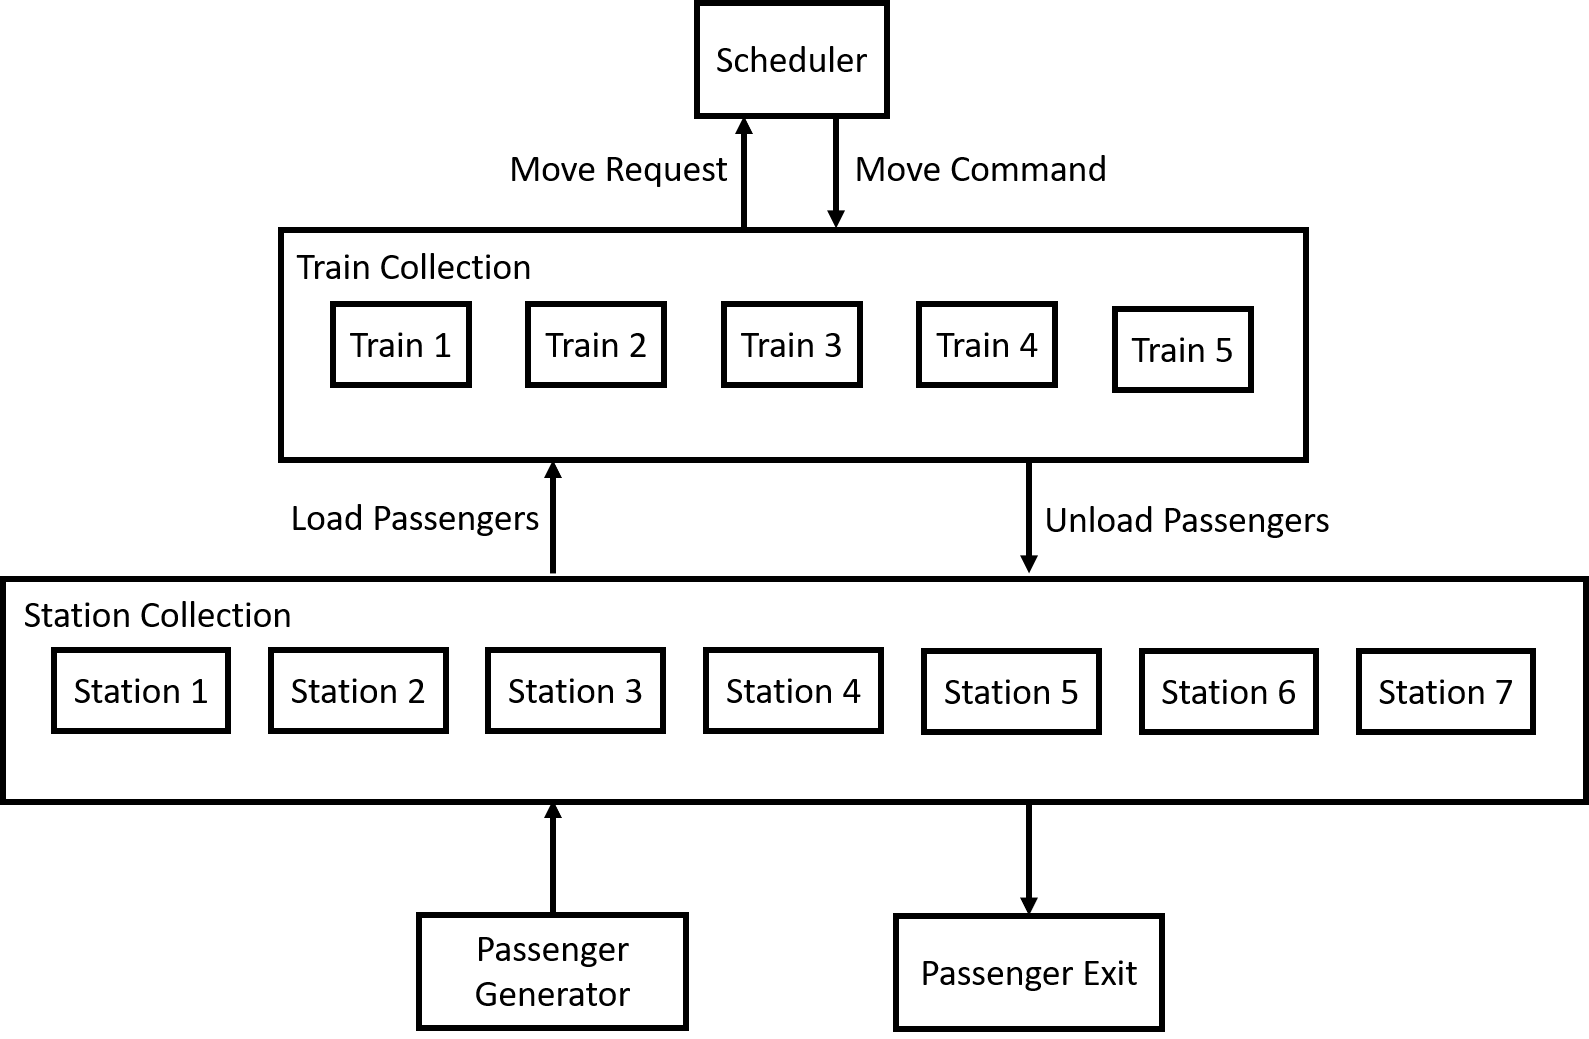
\includegraphics[width=6.5in]{hierarchy.png}
	\caption{Component Hierarchy}
	\label{fig:hierarchy}
\end{figure}
%
\subsection{Station Model}
The station serves as the creation and destruction point for passengers.  The station is also the only location where trains may load or unload passengers. The station is responsible for maintaining a pool of waiting passengers.  If a train does not have enough capacity to board all waiting passengers, then those passengers persist at the station and wait for the next train.  The inputs to the station are a pool of new passengers, an available passenger capacity by the current train, and a set of passengers to unload from the arriving train.  The outputs are a request to the current train for its available capacity after unloading passengers and a set of passengers to load onto the train. For its states, the station may be simply waiting, adding new passengers to the pool, receiving passengers from the train or providing passengers to the train.  It must also have a state variable that holds the current passenger collection.
\begin{align*}
DEVS_{\textrm{Station}} &= \left<X,Y,S,\delta_{ext},\delta_{int},\lambda,ta\right> \\
P &= Passenger\ Collection, |P|\in\mathbb{N}_0^+ \\
C &= \text{Passenger capacity of train} \\
X &= \lbrace(\text{``Unload Passengers''},\lbrace u|u\in\mathbb{N}_0\rbrace), \\ & (\text{``Remaining Capacity''},\lbrace c|c\in\mathbb{N}_0\rbrace), \\ &\lbrace P\rbrace\rbrace \\
Y &= \lbrace(\text{``Capacity Request''},()), \\ & (\text{``Load Passengers''},\lbrace\cup \emptyset p|p\in\mathbb{N}_0,p\leq C\rbrace)\rbrace \\
S_{action} &= \lbrace\text{waiting, adding passengers}, \\ & \text{receiving passengers, providing passengers}\rbrace \\
S_{passengers} &= \lbrace P, |P|\in\mathbb{N}_0^+\rbrace \\
S &= S_{action}\times S_{passengers} \\
\delta_{ext}(\text{waiting},e,(\text{''Unload Passsengers''},\lbrace u|u\in\mathbb{N}_0\rbrace)) &= (\text{receiving passengers},\lbrace u\rbrace) \\
\delta_{ext}(\text{waiting},e,(\text{``Remaining Capacity''},c)) &= (\text{providing passengers},p) \\
\delta_{int}(\text{waiting}) &= \text{waiting} \\
\delta_{int}(\text{waiting}) &= \text{adding passengers} \\
\delta_{int}(\text{adding passengers},\sigma) &= \text{waiting} \\
\lambda(\text{providing passengers}) &= (\text{``Load Passengers''},\lbrace p|p\in\mathbb{N}_0,p\leq C\rbrace) \\
ta &= \sigma \\
\end{align*}
%
\subsection{Track Section Model}

The track section model is needed to control access to track sections. A train
is permitted to enter a section if their is remaining capacity in the section.
When a train leaves a section the section's remaining capacity is increased by
one. The track section model can be represented by the DEVS with ports model 
below.

\newcommand{\InEnterReq}[0]{(\text{``Enter Request''}, ())}
\newcommand{\InExitReq}[0]{(\text{``Exit Request''}, ())}

\newcommand{\OutEnterRes}[1]{(\text{``Enter Response''}, #1)}

\begin{align*}
DEVS_{\textrm{Track}} &= \left<X,Y,S,\delta_{ext},\delta_{int},\lambda,ta\right> \\
    A &= \text{Number of trains allowed on section} \\
    X &= \{\InEnterReq, \\
        & \InExitReq
    \} \\
    Y &= \{\OutEnterRes{\{\text{May enter}, \text{May not enter}\}}\} \\
    S &= \{ a | a \in \mathbb{N}_0, a \leq A \} \\
    ta(S) &= \infty \\
    \delta_{ext}(a, e, \InEnterReq) &= 
        \begin{cases}
            a - 1 & \text{if\;} a > 0 \\
            a & \text{otherwise} \\
        \end{cases} \\
    \delta_{ext}(a, e, \InExitReq) &= 
        \begin{cases}
            a + 1 & \text{if\;} a < A \\
            a & \text{otherwise} \\
        \end{cases} \\
    \lambda(a) &= 
        \begin{cases}
            \text{May enter} & \text{if\;} a > 0 \\
            \text{May not enter} & \text{otherwise} \\
        \end{cases}
\end{align*}

\subsection{Train Model}

Trains travel station to station to unload and load passengers. Sometimes they
break down. They also follow a movement protocol and a loading and unloading
protocol. In the loading and unloading protocol, a train arrives at a station,
unloads some of its passengers, waits for a capacity request, responds with a
remaining capacity and awaits for the station to load the train. In the movement
protocol, the train asks the scheduler if it can be move forward and scheduler
replies with an accepted or rejected. Trains rejected from proceeding to the
next section still proceed as far as they can within their section. This
behavior is represented by the DEVS with ports model below. Any missing
transitions are assumed to return the input state. 

The model makes some simplifying assumptions. It assumes that each track section
includes stations and the track up to the next station. This assumption could be
relaxed by having the train keep track of whether or not the train is at a
station. A 50\% disembark rate is also assumed for unloading at each station. A
more detailed model would include each passengers destination station so that
forced breakdowns event would force passengers to exit and those that did not
reach their desired destination would board the next train (this model assumes
disembarkers never reboard). It also assumes that breakdown repair times and in
need of repair times are constant.

\newcommand{\InBreakDown}[0]{(\text{``Breakdown''}, ())}
\newcommand{\InCapReq}[0]{(\text{``Capacity Request''}, ())}
\newcommand{\InMoveRes}[1]{(\text{``Move Response''}, #1)}
\newcommand{\InLoadPassengers}[1]{(\text{``Load Passengers''}, #1)}

\newcommand{\OutRemainingCapacity}[1]{(\text{``Remaining Capacity''}, #1)}
\newcommand{\OutUnloadPassengers}[1]{(\text{``Unload Passengers''}, #1)}
\newcommand{\OutMoveReq}[1]{(\text{``Move Request''}, #1)}
\newcommand{\phase}[0]{\text{phase}}

\newcommand{\Mod}[2]{\mathrm{mod} (#1, #2)}

\begin{align*}
DEVS_{\textrm{Train}} &= \left<X,Y,S,\delta_{ext},\delta_{int},\lambda,ta\right> \\
    T &= \text{\# of trains} \\
    N &= \# \text{\;of train stations} \\
    C &= \text{Passenger capacity of train} \\
    m &= \text{Travel time from end of track} \\
        & \text{section to next section} \\
    X &= \{
      \InBreakDown, \\
      &  \InCapReq, \\
      &  \InLoadPassengers{\{ p | p \in \mathbb{N}_0, p \leq C \}} \\
      &  \InMoveRes{\{ \text{Accepted}, \text{Rejected} \}}
    \} \\
    Y &= \{
      \OutRemainingCapacity{\{ c | c \in \mathbb{N}_0 \}}, \\
      &  \OutUnloadPassengers{\{ u | u \in \mathbb{N}_0 \}}, \\
      &  \OutMoveReq{\\ 
        & \{ (i, t) | i \in \mathbb{N}_0, i < N, t \in \mathbb{N}_0, t < T \}}
    \} \\
    S_{action} &= \{
      \text{moving}, \text{needs repairs}, \text{in repair}, \\
      &  \text{loading}, \text{unloading}, \text{waiting for load}, \\
      &  \text{waiting for cap req} 
    \} \\
    S_{\text{position}} &= \{ i | i \in \mathbb{N}_0, i < N
    \} \\
    S_{passengers} &= \{ p | p \in \mathbb{N}_0, p \leq C \} \\
    S &= S_{action} \times S_{position} \times S_{passengers} \times \sigma \\
    ta(a, i, p, \sigma) &= \sigma \\
    %
    \delta_{ext}((\text{moving}, i, p, \sigma), e, \InBreakDown) &= 
        (\text{needs repair}, i, p, \\
        & \text{time till repairs start}) \\
    \delta_{ext}((\text{moving}, i, p, \sigma), e, \InMoveRes{\text{Accepted}})
        &= (\text{unloading}, \Mod{i+1}{N}, \ceil*{p/2}, \\
        & \text{loading time}) \\
    \delta_{ext}((\text{moving}, i, p, \sigma), e, \InMoveRes{\text{Rejected}})
        &= (\text{moving}, i, p, \max(m, \sigma - e)) \\
    \delta_{ext}((\text{waiting for cap req}, i, p, \sigma), e, \InCapReq) &=
        (\text{waiting for load}, i, p, \infty) \\
    \delta_{ext}((\text{waiting for load}, i, p, \sigma), e, \InLoadPassengers{p_{load}}) &=
        (\text{loading}, i, p + p_{load}, \text{loading time}) \\
    %
    \delta_{int}(\text{unloading}, i, p, \sigma) &= 
        (\text{waiting for cap req}, i, p, \infty) \\
    \delta_{int}(\text{loading}, i, p, \sigma) &= (\text{moving}, i, p,
        \text{time to next station}) \\
    \delta_{int}(\text{needs repair}, i, p, \sigma) &= 
        (\text{in repair}, i, p, \text{repair time}) \\
    \delta_{int}(\text{in repair}, i, p, \sigma) &= 
        (\text{moving}, i, p, \text{time to next station}) \\
    %
    \lambda(\text{moving}, i, p, \sigma) &= \OutMoveReq{(i, t)} \\ 
        & \text{\;where\;} t \text{\;is the constant train ID} \\
    \lambda(\text{unloading}, i, p, \sigma) &= \OutUnloadPassengers{\floor*{p/2}} \\
    \lambda(\text{waiting for cap req}, i, p, \sigma) &= \OutRemainingCapacity{C - p}
\end{align*}


\subsection{Scheduler Model}
A preliminary formal definition of the DEVS scheduler model is provided below. When a train is ready to resume moving it sends a move request in the form of its ID as in input to the scheduler.  Internally, the scheduler verifies whether or not it is safe to move.  It also identifies any trains currently waiting on the inquiring train.  It takes this collection of trains and outputs move commands to each.  In the case where no trains are able to move, the output is an empty set. The model remains in a perpetual state of waiting until it receives a move request from one of the trains.  It processes this request accordingly, responds, and then reverts back to a waiting state. The state consists of the two phases, waiting or moving trains, and state variables that store the input ID of the requesting train and its position.
\begin{align*} DEVS_{\textrm{Scheduler}} &= \left<X,Y,S,\delta_{ext},\delta_{int},\lambda,ta\right> \\
T &= \# \text{ of trains} \\
N &= \# \text{ of train stations} \\
X &= \lbrace\OutMoveReq{(i,t)|i\in\mathbb{N}_0,i<N, t\in\mathbb{N}_0,t<T}\rbrace \\
Y &= \lbrace\InMoveRes{(iset,tset)|iset\subseteq N, tset\subseteq T}\rbrace \cup\emptyset \\
S_{action} &= \lbrace \text{waiting, moving trains}\rbrace \\
S_{position} &= {i|i\in\mathbb{N}_0, i<N} \\
S_{train} &= {t|t\in\mathbb{N}_0, t<T} \\
S &= S_{action}\times S_{position}\times S_{train} \\
\delta_{ext}(\text{waiting},e,(\text{``Move Request''},i,t)) &= (\text{moving trains},i,t,\sigma) \\
\delta_{int}(\text{moving trains},i,t,\sigma) &= \text{waiting} \\
\delta_{int}(\text{waiting}) &= \text{waiting} \\
\lambda(\text{moving trains},i,t,\sigma) &= (\text{``Move Response''},\lbrace Accepted, Rejected\rbrace\times iset\times tset\cup \emptyset)\\
ta(\text{moving trains}) &= \sigma \\ 
ta(\text{waiting}) &= \infty \\
\end{align*}

\subsection{Planned Experiments}
The primary experiments will focus on disruptions in service due to train maintenance issues.  Given a train breakdown that causes a blockage on one of the tracks, we shall examine the effectiveness of a meet and pass routine.  Effectiveness shall be judged by the ability of the trains to pass by switching tracks without causing a deadlock, without causing significant delays in trains traveling in the opposite direction due to the track switching, and by monitoring passenger counts at the stations.  Monitoring the passenger counts is to evaluate that the service disruption does not cause a severe sustained surge in passengers waiting to board.  Another experiment will look at the effect of passenger surges at a given station, during rush hour for example, and the subway network's ability to maintain train movement given the increased loading and unloading times due to the surge. 

These experiments will also involve varying the number of trains in service, with the goal of finding the optimum number of trains particular to the subway circuit modeled.  An increase in the number of trains may nominally be able to carry a larger number of passengers, assuming the number of trains does not exceed the number of stations.  However, if a disruption occurs and a train is disabled, this can quickly lead to deadlock as there is no extra bandwidth in the rail system to allow the trains to switch and get around the disabled train because all stations are occupied at any given time.  Conversely, if there are too few trains operating it runs the risk of not having enough total capacity to carry the influx of passengers, even though it may be easier to overcome service disruptions.

\subsection{Expected Outcomes}

The subway simulation in this paper is designed to focus on two outcome variables: passenger wait times at stations and train delays. The expected outcome from this simulation is that increases in passing areas decreases train delays and a increased number of trains to service a subway line results in lower passenger wait times at stations.